\section{Response to Reviewer 10}
% \begin{bibunit}
\textbf{Reviewer 10---Major Contribution of the Paper---}\textit{%
This letter proposes a novel framework to address the issue of imperfect CSI in WNCS and presents solutions under both finite- and infinite-horizon LQR formulations.}\\[2mm]
\textbf{Authors' response:} \textcolor{black}{We truly appreciate the Reviewer's careful reading of our paper and valuable comments. In the revised version, we have carefully addressed the Reviewer's concerns and made the required modifications.}\\[4mm]
%%%
\textbf{Reviewer 10---Organization and Style---}\textit{%
The letter is well-organized and logically structured, but some descriptions could be more readable.
For example, in Part II, the paragraph beginning with ``Wireless receivers perform CSI measurements...'' could be improved by describing the signal flow explicitly: e.g., what information is transmitted from the sensor to the controller at time step $k$, then from the controller to the actuator, and how the detector provides the controller with the measured CSI from step $k-1$, etc.}\\[2mm]
\textbf{Authors' response:} \textcolor{black}{We thank the Reviewer for this valuable comment, which helped us improve the clarity of our letter. Due to space constraints, we could only provide a concise overview of the closed-loop system architecture in Fig. 1, which has been added to Section III in the revised version of the letter, immediately after describing the system model. The related excerpt of the revised version of the manuscript is included below for the Reviewer's convenience.}\\
\textcolor{blue}{Fig.~\ref{fig:architecture} summarizes this closed-loop system architecture.}
\begin{figure}[h!]
\begin{center}
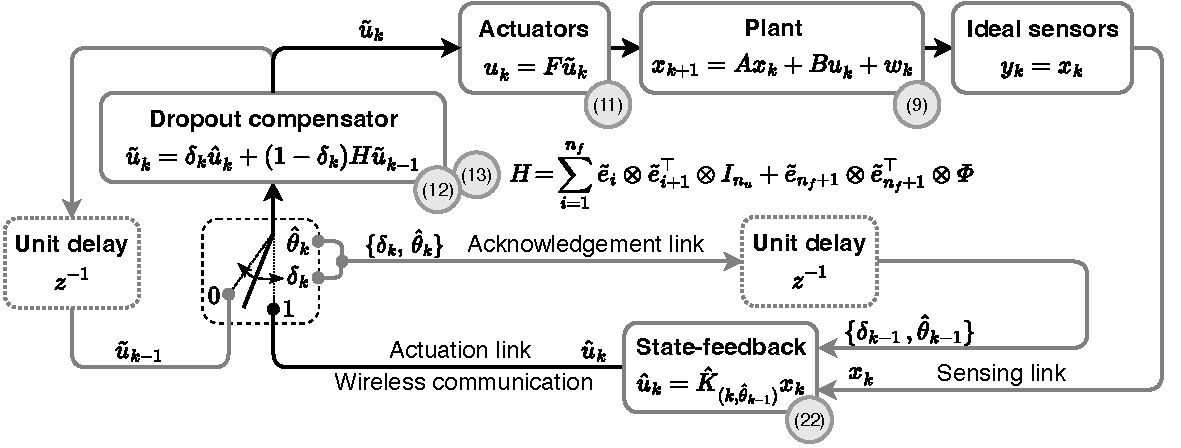
\includegraphics[width=0.8\columnwidth]{../wncs-lcss-cdc-25-architecture.pdf}
\caption{\textcolor{blue}{The closed-loop system architecture. The square blocks indicate the main components, and the shaded circles reference the related equations. A wireless link delivers SF control inputs to the actuators. The receiver measures the link state $\theta_k$ and communicates the measurement $\hat{\theta}_k$ with the transmission outcome $\delta_k$ to the controller. }}\label{fig:architecture}
\end{center}
\end{figure}\\[2mm]
%%%
\textbf{Reviewer 10---Technical Accuracy---1)}\textit{ %
Several variables are not explicitly defined in the text, such as $H^i$ in equation (23).}\\[2mm]
\textbf{Authors' response:} \textcolor{black}{We appreciate the Reviewer's feedback. We checked the manuscript for the definitions of the variables. $H$ refers to the message dropout compensation (MDC) scheme formalized by equation (13) and described in the text below the equation. Similar to $A^{h-i}$, $H^{i}$ in (23) indicates matrix exponentiation. It produces the following matrices.}
\begin{equation*}
    n_f = 0 \Rightarrow H^0 = I_{n_u},~H^1 = H = \mathit{\Phi},~H^2 = \mathit{\Phi}^{2},\dots,~H^i= \mathit{\Phi}^i~\forall i\in\mathbb{Z}^{0+}.
\end{equation*}
\begin{equation*}
    n_f = 1 \Rightarrow H^0 = \begin{bmatrix} I_{n_u} & 0 \\ 0 & I_{n_u} \end{bmatrix},~H^1 = H = \begin{bmatrix} 0 & I_{n_u} \\ 0 & \mathit{\Phi} \end{bmatrix},~H^2 = \begin{bmatrix} 0 & \mathit{\Phi} \\ 0 & \mathit{\Phi}^2 \end{bmatrix},\dots,
    ~H^i = \begin{bmatrix} 0 & \mathit{\Phi}^{i-1} \\ 0 & \mathit{\Phi}^i \end{bmatrix}~\forall i\in\mathbb{Z}^{+}.
\end{equation*}
\begin{equation*}
    n_f = 2 \Rightarrow H^0 =\! \begin{bmatrix} I_{n_u} & 0 & 0 \\ 0 & I_{n_u} & 0 \\ 0 & 0 & I_{n_u} \end{bmatrix}\!,~H^1 = H =\! \begin{bmatrix} 0 & I_{n_u} & 0 \\ 0 & 0 & I_{n_u} \\ 0 & 0 & \mathit{\Phi} \end{bmatrix}\!,\dots,
    ~H^i =\! \begin{bmatrix} 0 & 0 & \mathit{\Phi}^{i-2} \\ 0 & 0 & \mathit{\Phi}^{i-1} \\ 0 & 0 & \mathit{\Phi}^i \end{bmatrix}\!,
    ~\forall i\in\mathbb{Z}^{+}, i\geq 2. 
\end{equation*}
The explicit versions of $H^i$ matrices for $n_f>2$ follow the pattern defined by (13) and matrix multiplication. Due to the strict page limit of an L-CSS letter, we could not include any of these explicit forms in the revised version of the manuscript.\\[4mm]
%%%
\textbf{Reviewer 10---Technical Accuracy---2)}\textit{ %
In equation (5b), the summation over $\alpha_{i\mu}$ should
be with respect to $\mu$, not $i$, to ensure that the sum of the probabilities of all possible detector outputs given the true channel state $s_i$ is 1 --- consistent with the notation in equation (1).}\\[2mm]
\textbf{Authors' response:} \textcolor{black}{We are grateful to the Reviewer for this helpful observation. The Reviewer is correct: the summation over $\alpha_{i\mu}$ should be in $\mu$. We have corrected this typo in the revised version of the manuscript. This typo did not affect the other equations or the numerical implementation used to obtain the results in Section VIII. The revised equation (5b) version follows for the Reviewer's convenience.}
\begin{equation*}
   \mathbb{P}(\hat{\theta}_{k} = \hat{s}_{\mu} \mid \theta_{k} = s_i) = \alpha_{i\mu} \geq 0,~ \textcolor{blue}{\sum_{\mu=1}^M \alpha_{i\mu}= 1}.
\end{equation*}
\\[2mm]
%%%
\textbf{Reviewer 10---Technical Accuracy---3)}\textit{ %
Additionally, Part VIII does not specify whether the numerical example corresponds to the finite- or infinite-horizon case.}\\[2mm]
\textbf{Authors' response:} \textcolor{black}{We thank the Reviewer for the observation. This information is implicitly provided in the first sentence of the last paragraph of Section VIII: ``To compare the effects of transmitting several future control inputs on stability and control cost, we solve the LMIs (49) in the same setting.'' The state-feedback control gains are obtained by solving the LMIs (49), which refer to the infinite-horizon case addressed in Section VII. The stability issues also refer to the infinite-horizon setting, as discussed in Section VI. Unfortunately, we cannot explicitly indicate the infinite-horizon case without exceeding the rigid six-page limit of an L-CSS letter. On a side note, the finite-horizon state-feedback control for the baseline case of no future control inputs and perfect CSI is extensively validated by a statistically significant number of Monte Carlo simulations in [4].}\\[4mm]
%%%
\textbf{Reviewer 10---Technical Accuracy---4)}\textit{ %
In Figures 1 and 2, it's unclear why 3) is labeled as clusters while 4) is states. Since ``perfect" effectively corresponds to 4 clusters, perhaps the ordering should follow the degree of CSI quality: perfect, three, two, no CSI.}\\[2mm]
\textbf{Authors' response:} \textcolor{black}{We sincerely appreciate the Reviewer's pertinent comment. Because of the deadline for the initial submission and the rigid space constraints of an L-CSS letter, we have omitted details of the four scenarios analyzed in the numerical example. We integrated these details in the revised version of the letter, as reported below, for the Reviewer's convenience.}\\
``Fig. 3 shows the corresponding control costs in four selected scenarios: \textcolor{blue}{1) Perfect CSI; 2) Three measured states with thresholds $\{\hat{\beta_i}\}_{i=1}^{2} \!=\! \{-2.98,-2.08\}\,$dB and Gaussian CSI measurement noise having $\sigma_{\omega}^2=10^{-4}$; 3) Two clusters with a threshold $\hat{\beta}_1\!=\!-2.55\,$dB without CSI measurement noise; 4) No CSI.}''\\
\textcolor{black}{This information helps us to address the Reviewer's comment properly. The clusters refer to non-overlapping groups of states, i.e., disjoint sets of states. Thus, scenarios 1), 3), and 4) involve clusters. Specifically, the perfect CSI scenario 1) has $M=N=4$ and $P_e = I_N$, with four states belonging to separate clusters. Scenario 3) has the SINR threshold of $-2.55\,$dB, which coincides with the FSMC threshold $\beta_2$. Consequently, the first cluster comprises the FSMC states $s_1$ and $s_2$, while the second includes $s_3$ and $s_4$. The corresponding emission probability matrix (EPM) is 
\begin{equation*}
P_e=\begin{bmatrix}
1 & 0 \\ 1 & 0 \\ 0 & 1 \\ 0 & 1
\end{bmatrix}.
\end{equation*}
Scenario 4) has only one cluster with all FSMC states and $P_e=\bm{1}$. However, Scenario 2) has a detector with three output states, each including overlapping FSMC states owing to different SINR thresholds. Its EPM is 
\begin{equation*}
P_e=\begin{bmatrix}
1 & 0 & 0 \\ 0.337 & 0.663 & 0 \\ 0 & 0.613 & 0.387 \\ 0 & 0 & 1
\end{bmatrix}.
\end{equation*}
In conclusion, we have followed the Reviewer's suggestion and listed the scenarios in decreasing order of the detector's state number, from 4 to 1. As detailed above, the cluster keyword indicates a non-overlapping grouping of the FSMC states into sets and cannot be applied to the second scenario. For the Reviewer's convenience, we have reported the updated figures below. Please note a change in the long-run average costs because of the different process noise covariance requested by Reviewer 9.}
\begin{figure}[h!]
\begin{center}
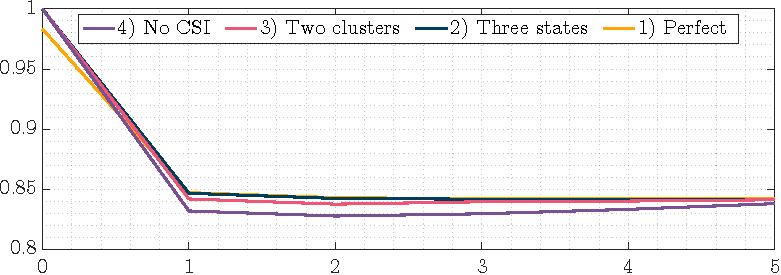
\includegraphics[width=0.76\columnwidth]{../stability-cntrl-a.pdf}
\caption{$\rho(\mathit{\Lambda})$ from (48) as a function of $n_f$.}\label{fig:stability}
\end{center}
\end{figure}
\begin{figure}[h!]
\begin{center}
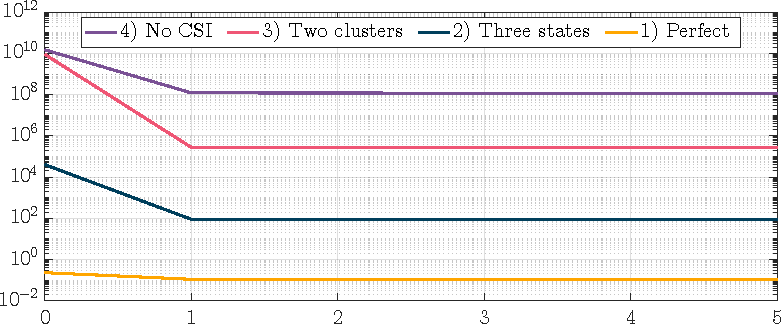
\includegraphics[width=0.76\columnwidth]{../cost-cntrl-a.pdf}
\caption{The long-run average cost $J_{\infty}^{\star}$ from (50b) as a function of $n_f$.}\label{fig:cost}
\end{center}
\end{figure}
\\[4mm]
%%%
\textbf{Reviewer 10---Technical Accuracy---5)}\textit{ %
The claim that ``one future control input provides the most significant improvement'' --- is this generally true?}\\[2mm]
\textbf{Authors' response:} \textcolor{black}{We thank the Reviewer for the question. All the considerations regarding $\rho(\mathit{\Lambda})$ and $J_{\infty}^{\star}$ values in Section VIII refer to the presented linearized model of a rotary inverted pendulum controlled over a specific FSMC and have no general validity, i.e., transmitting more than one future control input may be helpful in different settings. The theoretical results of this letter enable answering the question of the most suitable number of future control inputs to transmit for any linear plant, FSMC, EPM, and message dropout compensation matrix $\mathit{\Phi}$. Please see our response to Reviewer 9's second question on parameter tuning for an example that considers different values $\mathit{\Phi}$.
}\\[4mm]
%%%
\textbf{Reviewer 10---Technical Accuracy---6)}\textit{ %
If the four channel states had higher packet loss rates, could it be possible that sending more future control inputs would become more beneficial?}\\[2mm]
\textbf{Authors' response:} \textcolor{black}{We thank the Reviewer for the question. In principle, sending additional future control inputs may be more beneficial in scenarios with an exceptionally high message dropout rate. However, we did not find any examples supporting this. Our letter presented a setting with a high average message dropout probability (AMDP) of $9.075$\% and neglected the increase in dropout probability due to increased message length. As an example of the effects of the number of future control inputs that account for the message length increase and much higher average message dropout probabilities, consider the same plant model in a setting with $18$ Wi-Fi devices operating under saturated conditions, all located $7.5$ meters from the control message receiver, which is positioned $5$ meters away from the controller. The closed-loop control relies on the ISA-100.11a. Other parameters can be found in [12]. The resulting four-state Markov channels are as follows. The subscript index indicates the number of future control inputs that yield the reported TPM and the corresponding vectors of successful message delivery probabilities.
\begin{equation*}
    P_{c.0} = 
\begin{bmatrix}
0.232 & 0.025 & 0.030 & 0.713 \\
0.212 & 0.024 & 0.028 & 0.736 \\
0.210 & 0.024 & 0.028 & 0.738 \\
0.175 & 0.022 & 0.026 & 0.777
\end{bmatrix},~
\hat{\delta}_{.0} = 
\begin{bmatrix}
0.022 \\ 0.374 \\ 0.633 \\ 0.991
\end{bmatrix}^{\top},~\text{AMDP}_{0} = 21.418\%.
\end{equation*}
\begin{equation*}
    P_{c.1} = 
\begin{bmatrix}
0.236 & 0.025 & 0.029 & 0.710 \\
0.216 & 0.024 & 0.028 & 0.732 \\
0.213 & 0.024 & 0.028 & 0.735 \\
0.179 & 0.021 & 0.025 & 0.775
\end{bmatrix},~
\hat{\delta}_{.1} = 
\begin{bmatrix}
0.021 \\ 0.374 \\ 0.633 \\ 0.991
\end{bmatrix}^{\top},~\text{AMDP}_{1} = 21.798\%.
\end{equation*}
\begin{equation*}
    P_{c.2} = 
\begin{bmatrix}
0.240 & 0.025 & 0.029 & 0.706 \\
0.220 & 0.024 & 0.028 & 0.728 \\
0.217 & 0.023 & 0.028 & 0.732 \\
0.182 & 0.021 & 0.025 & 0.772
\end{bmatrix},~
\hat{\delta}_{.2} = 
\begin{bmatrix}
0.020 \\ 0.374 \\ 0.633 \\ 0.991
\end{bmatrix}^{\top},~\text{AMDP}_{2} = 22.132\%.
\end{equation*}
\begin{equation*}
    P_{c.3} = 
\begin{bmatrix}
0.243 & 0.024 & 0.029 & 0.704 \\
0.223 & 0.023 & 0.028 & 0.726 \\
0.220 & 0.023 & 0.027 & 0.730 \\
0.185 & 0.021 & 0.025 & 0.769
\end{bmatrix},~
\hat{\delta}_{.3} = 
\begin{bmatrix}
0.020 \\ 0.374 \\ 0.633 \\ 0.991
\end{bmatrix}^{\top},~\text{AMDP}_{3} = 22.430\%.
\end{equation*}
\begin{equation*}
    P_{c.4} = 
\begin{bmatrix}
0.246 & 0.024 & 0.028 & 0.702 \\
0.226 & 0.023 & 0.027 & 0.724 \\
0.223 & 0.023 & 0.027 & 0.727 \\
0.188 & 0.021 & 0.025 & 0.766
\end{bmatrix},~
\hat{\delta}_{.4} = 
\begin{bmatrix}
0.019 \\ 0.374 \\ 0.633 \\ 0.991
\end{bmatrix}^{\top},~\text{AMDP}_{4} = 22.699\%.
\end{equation*}
\begin{equation*}
    P_{c.5} = 
\begin{bmatrix}
0.249 & 0.024 & 0.028 & 0.699 \\
0.228 & 0.023 & 0.027 & 0.722 \\
0.225 & 0.023 & 0.027 & 0.725 \\
0.190 & 0.021 & 0.025 & 0.764
\end{bmatrix},~
\hat{\delta}_{.5} = 
\begin{bmatrix}
0.019 \\ 0.374 \\ 0.633 \\ 0.991
\end{bmatrix}^{\top},~\text{AMDP}_{5} = 22.945\%.
\end{equation*}
Consider the four scenarios of the letter previously discussed in response to the fourth Reviewer's comment on technical accuracy. 
Figures \ref{fig:stability-coeff-x} and \ref{fig:cost-cntrl-x} illustrate the stability and long-run average cost in the presented setting, with a process noise covariance $\Sigma_w \!=\! 4\cdot 10^{-6} I_4$. Similar to the setting of the letter, transmitting one future control input offers the most significant benefit regarding stability and control cost. Transmitting two control inputs reduces $\rho(\mathit{\Lambda})$ but increases $J_{\infty}^{\star}$ compared to transmitting one future control input. 
The results concerning the fourth scenario of no CSI are limited to three future control inputs, as sending four or more future control inputs leads to instability in the closed-loop system due to extremely high message dropout rates indicated by AMDP values exceeding $22.5$\%. The values of $\rho(\mathit{\Lambda})$ become $38.543$ and $50.569$, which indicate highly unstable behavior with infinite cost. Theorem 5 is applicable only to stabilizable systems, meaning that the values of $J_{\infty}^{\star}$ cannot be obtained using (50b) for the fourth scenario of no CSI with more than three future control inputs. Due to the page limit of an L-CSS letter, we could not include these details in the revised version of the manuscript.
\begin{figure}[h!]
\begin{center}
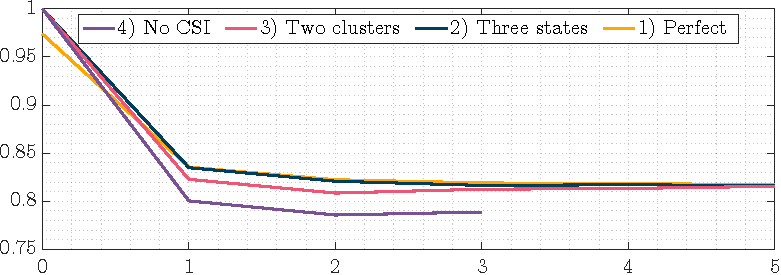
\includegraphics[width=0.76\columnwidth]{stability-cntrl-x.pdf}
\caption{The spectral radius of the mean-square stability verification matrix, $\rho(\mathit{\Lambda})$, as a function of the number of control inputs $n_f$ for the rotary inverted pendulum under the proposed infinite-horizon linear–quadratic regulation (LQR) with the dropout compensation factor $\mathit{\Phi}=0.1$ and FSMCs 1–5 described above.}\label{fig:stability-coeff-x}
\end{center}
\end{figure}
\begin{figure}[h!]
\begin{center}
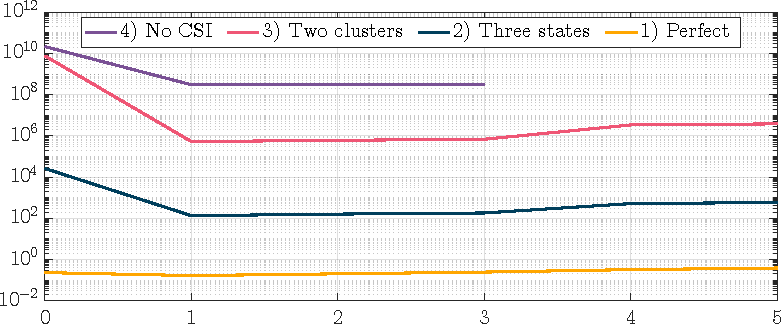
\includegraphics[width=0.76\columnwidth]{cost-cntrl-x.pdf}
\caption{The long-run average cost, $J_{\infty}^{\star}$, as a function of the number of control inputs $n_f$ for the rotary inverted pendulum under the proposed infinite-horizon linear–quadratic regulation (LQR) with the dropout compensation factor $\mathit{\Phi}=0.1$ and FSMCs 1–5 described above.}\label{fig:cost-cntrl-x}
\end{center}
\end{figure}
}\\[4mm]
%%%
\textbf{Reviewer 10---Technical Accuracy---7)}\textit{ %
Regarding the statement ``The control law without CSI performs worse regarding control costs but benefits the most from a future control input''---doesn't Figure 2 show that the ``two-cluster'' case benefits more than the ``no CSI'' case?}\\[2mm]
\textbf{Authors' response:} \textcolor{black}{We are thankful to the Reviewer for a thoughtful observation. The considered statement referred to Fig. 1 in the previous version of the manuscript, which is now Fig. 2 in the revised version of the letter, since the no CSI case has the greatest improvement in terms of $\rho(\mathit{\Lambda})$. Please note that we removed this statement to make room for the details on all four selected scenarios and the new Fig. 1, which clarifies the closed-loop system architecture. The final observations on the numerical results in Figs. 2 and 3 are reported below for the Reviewer’s convenience.}\\
\textcolor{blue}{All scenarios show that transmitting one future control input significantly improves stability and control costs, while more accurate and detailed CSI always reduces control costs.}\\[4mm]
%%%
\textbf{Reviewer 10---Presentation---}\textit{%
In Part III, the sentence ``Similarly to [4], [5]...'' should be revised. ``similarly'' $\to$ ``similar''.}\\[2mm]
\textbf{Authors' response:} \textcolor{black}{We thank the Reviewer for the valuable suggestion. We have implemented it.}\\[4mm]
%%%
\textbf{Reviewer 10---Adequacy of Citations---}\textit{%
The citations appear to be adequate.}\\[2mm]
\textbf{Authors' response:} \textcolor{black}{We are grateful to the Reviewer for the valuable feedback.}\\[4mm]
%%%
\textbf{Authors' concluding remark:} \textcolor{black}{We are thankful to the Reviewer for the valuable comments and suggestions. We sincerely hope the above explanations have adequately addressed the Reviewer's concerns.}
% \putbib
% \end{bibunit}